%%%------------------------------------------------------------------------------------%%
%%%------------------------------------------------------------------------------------%%
%%% Content: Open-Science-Paper LaTeX Scaffold 
%%% Usage: Collaborative scientific paper writing 
%%% Author: Claas-Thido Pfaff
%%%------------------------------------------------------------------------------------%%
%%%------------------------------------------------------------------------------------%%

%%%------------------------------------------------------------------------------%%%
%%% Document class: open_science_paper (Based on Koma-Script: article) %%%
%%%------------------------------------------------------------------------------%%%
%%
%

\documentclass[color=false, csvdata=false]{ost/subdocuments/open_science_thesis}\usepackage{graphicx, color}
%% maxwidth is the original width if it is less than linewidth
%% otherwise use linewidth (to make sure the graphics do not exceed the margin)
\makeatletter
\def\maxwidth{ %
  \ifdim\Gin@nat@width>\linewidth
    \linewidth
  \else
    \Gin@nat@width
  \fi
}
\makeatother

\IfFileExists{upquote.sty}{\usepackage{upquote}}{}
\definecolor{fgcolor}{rgb}{0.2, 0.2, 0.2}
\newcommand{\hlnumber}[1]{\textcolor[rgb]{0,0,0}{#1}}%
\newcommand{\hlfunctioncall}[1]{\textcolor[rgb]{0.501960784313725,0,0.329411764705882}{\textbf{#1}}}%
\newcommand{\hlstring}[1]{\textcolor[rgb]{0.6,0.6,1}{#1}}%
\newcommand{\hlkeyword}[1]{\textcolor[rgb]{0,0,0}{\textbf{#1}}}%
\newcommand{\hlargument}[1]{\textcolor[rgb]{0.690196078431373,0.250980392156863,0.0196078431372549}{#1}}%
\newcommand{\hlcomment}[1]{\textcolor[rgb]{0.180392156862745,0.6,0.341176470588235}{#1}}%
\newcommand{\hlroxygencomment}[1]{\textcolor[rgb]{0.43921568627451,0.47843137254902,0.701960784313725}{#1}}%
\newcommand{\hlformalargs}[1]{\textcolor[rgb]{0.690196078431373,0.250980392156863,0.0196078431372549}{#1}}%
\newcommand{\hleqformalargs}[1]{\textcolor[rgb]{0.690196078431373,0.250980392156863,0.0196078431372549}{#1}}%
\newcommand{\hlassignement}[1]{\textcolor[rgb]{0,0,0}{\textbf{#1}}}%
\newcommand{\hlpackage}[1]{\textcolor[rgb]{0.588235294117647,0.709803921568627,0.145098039215686}{#1}}%
\newcommand{\hlslot}[1]{\textit{#1}}%
\newcommand{\hlsymbol}[1]{\textcolor[rgb]{0,0,0}{#1}}%
\newcommand{\hlprompt}[1]{\textcolor[rgb]{0.2,0.2,0.2}{#1}}%

\usepackage{framed}
\makeatletter
\newenvironment{kframe}{%
 \def\at@end@of@kframe{}%
 \ifinner\ifhmode%
  \def\at@end@of@kframe{\end{minipage}}%
  \begin{minipage}{\columnwidth}%
 \fi\fi%
 \def\FrameCommand##1{\hskip\@totalleftmargin \hskip-\fboxsep
 \colorbox{shadecolor}{##1}\hskip-\fboxsep
     % There is no \\@totalrightmargin, so:
     \hskip-\linewidth \hskip-\@totalleftmargin \hskip\columnwidth}%
 \MakeFramed {\advance\hsize-\width
   \@totalleftmargin\z@ \linewidth\hsize
   \@setminipage}}%
 {\par\unskip\endMakeFramed%
 \at@end@of@kframe}
\makeatother

\definecolor{shadecolor}{rgb}{.97, .97, .97}
\definecolor{messagecolor}{rgb}{0, 0, 0}
\definecolor{warningcolor}{rgb}{1, 0, 1}
\definecolor{errorcolor}{rgb}{1, 0, 0}
\newenvironment{knitrout}{}{} % an empty environment to be redefined in TeX

\usepackage{alltt} 

%% Available class options [defaults]
% - color true/[false]: Changes between colored output and a black and white theme 
% - csvdata true/[false]: With csv data enabled you can use the csv file under
%   the data folder to insert title header information into the document.
% - gitinfo true/[false]: Include git information into the title header of the 
%   document. This requires the setup of git hooks which you can do by issuing 
%   the make task (make githooks). After that you need to specify the url of the 
%   git repository inside of the style file and you are done.
% - print true/[false] switches between the color model rgb which is optimal for displays 
%   and the cmyk color model which is required for professional printing. 
% - linenumbers true/[false]: Switch on/off line numbers for the whole document.
% - sectionnumbers true/[false]: Switch between numbered and numberless sections 
% - autolayout [true]/false: Switch between the nice automatic calculated typearea layout 
%   (Koma script) and a fixed geometry page layout (geometry package). You need to set the 
%   geometry inside of the style file if you choose false. 
% - twosidelayout true/[false]: Switch between two and one side page layout.
% - reversepagelayout [false]/true reverse the order of odd and even side margins. This 
%   option can be used to start the paper on a left or right page. 
% - resetdefaultclassoptions true/[false] resets the default options the open science paper 
%   loads the scrartcl class. After that you can modify every option via the open science 
%   paper class call. For example to change the calculated typearea you can use 
%   \documentclass[resetdefaultclassoptions=true, DIV=7]{ost/subdocuments/open_science_paper}  
% - parindent true/[false] Switch paragraph indent on or off.

%%%------------------------------------------------------------------------------%%%
%%% Load user options %%%
%%%------------------------------------------------------------------------------%%%

%%%------------------------------------------------------------------------------------%%
%%%------------------------------------------------------------------------------------%%
%%% Content : Open-Science-Paper LateX-Style 
%%% Use : Open-Sciene-Paper user modifications 
%%% Author : Claas-Thido Pfaff
%%%------------------------------------------------------------------------------------%%
%%%------------------------------------------------------------------------------------%%

%%%-------------------------------------------------%%%
%%% Define your papers geometry %%%
%%%-------------------------------------------------%%%

%% Note: 

% Needs the class option autolayout=false

%% Example:

% \geometry{left=4cm, right=4cm, textheight=25cm}

%% Note: 

% Find all available options in the geometry package 
% documentation.

%%%-------------------------------------------------%%%
%%% Define own colors %%%
%%%-------------------------------------------------%%%

%% Example:

% \xdefinecolor{YourColor}{rgb}{0,0,0.7}

%%%-------------------------------------------------%%%
%%% Define own commands %%%
%%%-------------------------------------------------%%%

%% Example:

% \newcommand{name}[number of parameters]{things to do}

%%%-------------------------------------------------%%%
%%% Define own environments %%%
%%%-------------------------------------------------%%%

%% Example:

% \newenvironment{name}[number of parameters]{definition begin}{definition end}

%%%-------------------------------------------------%%%
%%% Define titlel authors and affiliation %%%
%%%-------------------------------------------------%%%

%% Note: You can set them empty to remove the line

% \ospSetTitle{This is the title of the paper}  
% \ospSetAuthors{Author one\textsuperscript{1,2,a}, Author two\textsuperscript{2,b}}  
% \ospSetContacts{foo@bar.com\textsuperscript{a}, bar@foo.com\textsuperscript{b}}
% \ospSetAffiliations{University of XY departement of Z\textsuperscript{1}, University of \ldots}
% \ospSetKeywords{Open Science, Git, R, Knitr, ggplot2, tikz}

% \ospSetTitleKeywordContactName{Cont:}
% \ospSetTitleKeywordAffiliationName{Affi:}
% \ospSetTitleKeywordName{Keys:}

%% Fonts 

% \ospSetFontTitle{\normalfont\sffamily\Huge\bfseries} 

%% Lengths [default]

% \setlength{\ospLengtTitleLogoColwidth}{0.2\textwidth} %[0.23\textwidth]
% \setlength{\ospLengtTitleTitleColwidth}{0.5\textwidth} %[0.55\textwidth] 
% \setlength{\ospLengtTitleSpaceAbove}{2\baselineskip} %[0.01\baselineskip] 
% \setlength{\ospLengtTitleSpaceBelow}{-1\baselineskip} %[0.01\baselineskip] 

%%%-------------------------------------------------%%%
%%% Define document column count %%%
%%%-------------------------------------------------%%%

% \ospSetColumnCount{1}

%%%-------------------------------------------------%%%
%%% Define footer contents and styling %%%
%%%-------------------------------------------------%%%

%% Contents

% \ospSetFooterTextRightOfSeparator{Right of separator} 
% \ospSetFooterTextSeparator{xx} 
% \ospSetFooterTextLeftOfSeparator{Left of separator} 
% \ospSetFullLeftFooter{I am the complete left footer}
% \ospSetFullRightFooter{\textbf{\thepage}}

%% Colors

% \ospSetFooterRuleColor{YourColor}
% \ospSetFooterPageNumberingColor{DarkOrange} 

%% Lengths [default]

% \setlength{\ospLengthFooterRuleWidth}{5pt} %[0.3pt]
% \setlength{\ospLengthHeaderRuleWidth}{0pt} %[0pt] 

%%%-------------------------------------------------%%%
%%% Set and change the git info display  %%%
%%%-------------------------------------------------%%%

%% Note 
% This features need the gitinfo class option set 
% inside the root file.

% \ospSetGitUrl{\url{www.....}}
% \ospSetGitInfoLine{}

%%%-------------------------------------------------%%%
%%% Set PDF options %%%
%%%-------------------------------------------------%%%

%% Example:
%  \hypersetup{%
%   pdfauthor={Your-Name},
%   pdfcreator={Your-Name},
%   pdfsubject={Subject},
%   pdfkeywords={Keyword1, Keyword2, ...}
%  }

%% Note: 
% See the hyperref package documentation for more options

%%%-------------------------------------------------%%%
%%% Bibliography options %%%
%%%-------------------------------------------------%%%

\ExecuteBibliographyOptions{%
url=false,%
isbn=false,%
doi=false,%
firstinits=false,%
bibencoding=utf8%
} 

% Add a BibTeX bibliography file 
\addbibresource{usr/subdocuments/open_science_thesis.bib}
 

%%%------------------------------------------------------------------------------%%%
%%% Begin the document %%%
%%%------------------------------------------------------------------------------%%%

\begin{document}

%%%--------------------------------------------------------------%%%
%%% Document preparations %%%
%%%--------------------------------------------------------------%%%
%%
%

%%%-------------------------------------------------%%%
%%% Preferences for Knitr %%%
%%%-------------------------------------------------%%%


%%%-------------------------------------------------%%%
%%% Sub document global preferences for Knitr %%%
%%%-------------------------------------------------%%%






%%%--------------------------------------------------------------%%%
%%% Document content %%%
%%%--------------------------------------------------------------%%%
%%
%

%%%-------------------------------------------------%%%
%%% Include header %%%
%%%-------------------------------------------------%%%


%%%-------------------------------------------------%%%
%%% Sub document header %%%
%%%-------------------------------------------------%%% 

\ostMakeTitle



%%%-------------------------------------------------%%%
%%% Include abstract %%%
%%%-------------------------------------------------%%%


%%%-------------------------------------------------%%%
%%% Sub document abstract %%%
%%%-------------------------------------------------%%%

\begin{abstract}

% Remove the lipsum and fill in your abstract text here
\lipsum[1]

\end{abstract}





%%%-------------------------------------------------%%%
%%% Include introduction %%%
%%%-------------------------------------------------%%%


%%%-------------------------------------------------%%%
%%% Sub document introduction %%%
%%%-------------------------------------------------%%%

\section{Introduction}

% Remove the lipsum and the list example and fill in your introduction text here
\capital{T} his is just an introduction text snippet to show how drop caps look in this document.
\lipsum[1]

\begin{itemize}
	\item One
		\begin{itemize}
			\item One One
				\begin{itemize}
					\item One One One
				\end{itemize}
		\end{itemize}
	\item Two
	\item Three
\end{itemize}

\lipsum[1-2]




%%%-------------------------------------------------%%%
%%% Include material and methods %%%
%%%-------------------------------------------------%%%


%%%-------------------------------------------------%%%
%%% Sub document for material and methods %%%
%%%-------------------------------------------------%%%

\section{Material And Methods}

% Remove the lipsum and example table fill in your material and methods text here


\lipsum[1]


% example for a one column table %

\begin{table}[H] % {{{
% Label tab:test_table_one
	\centering
	\label{tab:test_table_one}
	\caption{Lorem ipsum dolor sit amet, consectetuer adipiscing elit. Aenean
	 commodo ligula eget dolor. Aenean massa. Cum sociis natoque penatibus et magnis
	 dis parturient montes, nascetur ridiculus mus. Donec quam felis, ultricies nec,
	 pellentesque eu, pretium quis, sem.}
	   {\small
			\begin{tabular}{p{0.055\columnwidth}p{0.055\columnwidth}p{0.055\columnwidth}p{0.055\columnwidth}p{0.055\columnwidth}p{0.055\columnwidth}p{0.055\columnwidth}p{0.055\columnwidth}p{0.055\columnwidth}}
				\toprule
					A & B & C & D & E & F & G & H & I\\ 
				\midrule
					1 & 2 & 3 & 4 & 5 & 6 & 7 & 8 & 9\\ 
					1 & 2 & 3 & 4 & 5 & 6 & 7 & 8 & 9\\ 
					1 & 2 & 3 & 4 & 5 & 6 & 7 & 8 & 9\\ 
				\bottomrule
			\end{tabular}
		}
\end{table} % }}}


\lipsum[1]



%%%-------------------------------------------------%%%
%%% Include results %%%
%%%-------------------------------------------------%%%


%%%-------------------------------------------------%%%
%%% Sub document results %%%
%%%-------------------------------------------------%%%

\section{Results}

% Remove the lipsum and the example plots and tables to fill in your abstract text here

\subsection{Subheading}

\lipsum[1-2]

\begin{figure}[H] % {{{
   \centering
      \begin{tikzpicture}
	 \node[pictureframe]{%    
	    \begin{minipage}{0.47\textwidth}%
	       \begin{center}
\begin{knitrout}
\definecolor{shadecolor}{rgb}{0.969, 0.969, 0.969}\color{fgcolor}
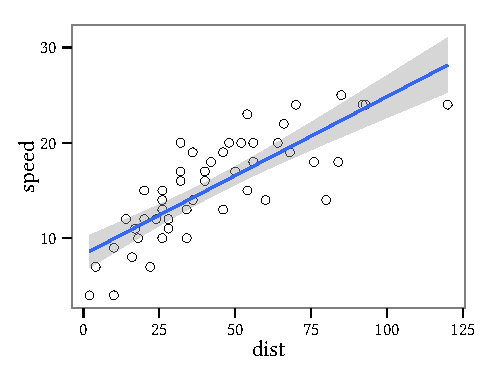
\includegraphics[width=\maxwidth]{usr/graphics/dynamic/test_plot} 

\end{knitrout}

	       \end{center}
	    \end{minipage}
	 };
      \end{tikzpicture}
   \caption{Lorem ipsum dolor sit amet, consectetuer adipiscing elit. Aenean
   commodo ligula eget dolor. Aenean massa. Cum sociis natoque penatibus et magnis
   dis parturient montes, nascetur ridiculus mus. Donec quam felis, ultricies nec,
   pellentesque eu, pretium quis, sem.}
\label{fig:test_plot}
\end{figure} % }}}

\lipsum 

\begin{equation}
   \sqrt[3]{1-y^2}
\end{equation}

\setlength\multlinegap{0pt}
\begin{multline} \tag{2}
   \sum_{t \in \mathbf{T}} \int_a^t
   \biggl\lbrace \int_a^t f(t - x)^2 \,
   g(y)^2 \,dx \biggr\rbrace \,dy \\
   = \sum_{t \notin \mathbf{T}} \int_t^a
   \biggl\lbrace g(y)^2 \int_t^a
   f(x)^2 \,dx \biggr\rbrace \,dy
\end{multline}

\begin{figure*} % {{{
   \centering
      \begin{tikzpicture}
	 \node[pictureframe]{%    
	    \begin{minipage}{0.98\textwidth}%
	       \begin{center}
\begin{knitrout}
\definecolor{shadecolor}{rgb}{0.969, 0.969, 0.969}\color{fgcolor}
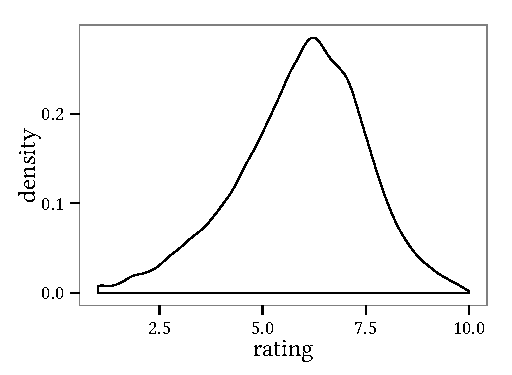
\includegraphics[width=\maxwidth]{usr/graphics/dynamic/test_plot_two1} 
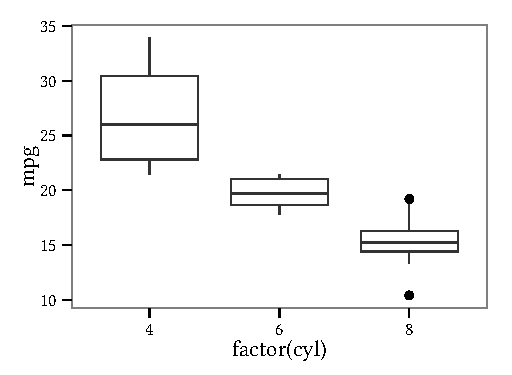
\includegraphics[width=\maxwidth]{usr/graphics/dynamic/test_plot_two2} 

\end{knitrout}

	       \end{center}
	    \end{minipage}
	 };
      \end{tikzpicture}
   \caption{Lorem ipsum dolor sit amet, consectetuer adipiscing elit. Aenean
   commodo ligula eget dolor. Aenean massa. Cum sociis natoque penatibus et magnis
   dis parturient montes, nascetur ridiculus mus. Donec quam felis, ultricies nec,
   pellentesque eu, pretium quis, sem.}
\label{fig:test_plot_two}
\end{figure*} % }}}

\lipsum[1-4]

\begin{lstlisting}[language=Ruby]
#!/usr/bin/ruby

$i = 0
$num = 5

while $i < $num  do
   puts("Text inside the loop: i = #$i")
   $i +=1
end
\end{lstlisting}

% example for a two column table %

\begin{table*} % {{{
% Label tab:test_plot_two 
	\centering
	\label{tab:test_table_two}
	\caption{Lorem ipsum dolor sit amet, consectetuer adipiscing elit. Aenean
	 commodo ligula eget dolor. Aenean massa. Cum sociis natoque penatibus et magnis
	 dis parturient montes, nascetur ridiculus mus. Donec quam felis, ultricies nec,
	 pellentesque eu, pretium quis, sem.}
	   {\small
		\begin{tabular}{p{0.08\textwidth}p{0.08\textwidth}p{0.08\textwidth}p{0.08\textwidth}p{0.08\textwidth}p{0.08\textwidth}p{0.08\textwidth}p{0.08\textwidth}p{0.08\textwidth}}
				\toprule
				   \multicolumn{4}{c}{A-D}   & \multicolumn{5}{c}{E-I}\\
				\cmidrule(lr){1-4} \cmidrule(lr){5-9}
					A     & B & C & D & E & F & G & H & I\\
				\midrule
					1     & 2 & 3 & 4 & 5 & 6 & 7 & 8 & 9\\
					1     & 2 & 3 & 4 & 5 & 6 & 7 & 8 & 9\\
					1     & 2 & 3 & 4 & 5 & 6 & 7 & 8 & 9\\
					1     & 2 & 3 & 4 & 5 & 6 & 7 & 8 & 9\\
				\bottomrule
			\end{tabular}
		}
\end{table*} % }}}






%%%-------------------------------------------------%%%
%%% Include discussion %%%
%%%-------------------------------------------------%%%


%%%-------------------------------------------------%%%
%%% Sub document for discussion %%%
%%%-------------------------------------------------%%%

\section{Discussion}

% Remove the lipsum and fill in your discussion text here
\lipsum[1-4]



%%%-------------------------------------------------%%%
%%% Include acknowledgements %%%
%%%-------------------------------------------------%%%


%%%-------------------------------------------------%%%
%%% Sub document for acknowledgement %%%
%%%-------------------------------------------------%%%

\section{Acknowledgements}

% Remove the lipsum and fill in your acknowledgements here
\lipsum[4-5]



%%%-------------------------------------------------%%%
%%% Include the bibliography %%%
%%%-------------------------------------------------%%%


%%%-------------------------------------------------%%%
%%% Sub document bibliography inclusion %%%
%%%-------------------------------------------------%%%

\section{References}

\nocite{*}
\printbibliography



%%%------------------------------------------------------------------------------%%%
%%% End of document %%%
%%%------------------------------------------------------------------------------%%%

\end{document}
